\documentclass{beamer}
\usetheme{Madrid}

\usepackage[utf8]{inputenc}
\usepackage[russian]{babel}
%\usepackage{hyperref}
%\usepackage[noline, noend, onelanguage, boxed]{algorithm2e}
\setcounter{MaxMatrixCols}{20}

\title[]{Реализация нейронной сети, выполняющей декодирование кода~Хэмминга с~использованием технологии Google Colaboratory}
\author[Архипов А.\,Е.]{Архипов~Антон~Евгеньевич}
\institute[ЮФУ~ИММиКН]{Прикладная математика и информатика \\
Кафедра алгебры и дискретной математики \\
Научный руководитель: к.т.н.~Мкртичян~Вячеслав~Виталиевич \\
}
\date{Июнь 2018}

\begin{document}

\begin{frame}
  \titlepage
\end{frame}

%\begin{frame}{Содержание}
%  \tableofcontents
%  % You might wish to add the option [pausesections]
%\end{frame}


\begin{frame}{Цели работы}
    \begin{itemize}
  \item {
    Построить реализацию нейронной сети, выполняющей декодирование кода~Хэмминга с~использованием технологии Google Colaboratory.
  }
  \item {
    Обеспечить вероятность выдачи корректного результата работы нейронной сети, выполняющей декодирование кода Хэмминга с~использованием технологии Google Colaboratory не~менее~0.85.
  }
  \end{itemize}
\end{frame}



\begin{frame}{Код Хэмминга}
Выберем код Хэмминга $\mathbb{C}(n=16, k=11)$ с пораждающей матрицей
\begin{equation}
\nonumber
G =
\begin{pmatrix}
0 & 0 & 0 & 0 & 0 & 0 & 0 & 0 & 1 & 0 & 0 & 1 & 1 & 0 & 1 & 0 \\
0 & 0 & 0 & 0 & 0 & 0 & 1 & 0 & 0 & 0 & 0 & 0 & 1 & 0 & 1 & 1 \\
0 & 0 & 0 & 0 & 0 & 1 & 0 & 0 & 0 & 0 & 0 & 0 & 1 & 1 & 0 & 1 \\
0 & 0 & 0 & 0 & 1 & 0 & 0 & 0 & 0 & 0 & 0 & 0 & 1 & 1 & 1 & 0 \\
0 & 0 & 0 & 1 & 0 & 0 & 0 & 0 & 0 & 0 & 0 & 1 & 0 & 0 & 1 & 1 \\
0 & 0 & 1 & 0 & 0 & 0 & 0 & 0 & 0 & 0 & 0 & 1 & 0 & 1 & 0 & 1 \\
0 & 1 & 0 & 0 & 0 & 0 & 0 & 0 & 0 & 0 & 0 & 1 & 0 & 1 & 1 & 0 \\
1 & 0 & 0 & 0 & 0 & 0 & 0 & 0 & 0 & 0 & 0 & 1 & 1 & 0 & 0 & 1 \\
0 & 0 & 0 & 0 & 0 & 0 & 0 & 1 & 0 & 0 & 0 & 0 & 0 & 1 & 1 & 1 \\
0 & 0 & 0 & 0 & 0 & 0 & 0 & 0 & 0 & 1 & 0 & 1 & 1 & 1 & 0 & 0 \\
0 & 0 & 0 & 0 & 0 & 0 & 0 & 0 & 0 & 0 & 1 & 1 & 1 & 1 & 1 & 1
\end{pmatrix}
\end{equation}
\end{frame}









\begin{frame}{Нейронные сети}
\begin{figure}[h]
    \centering
  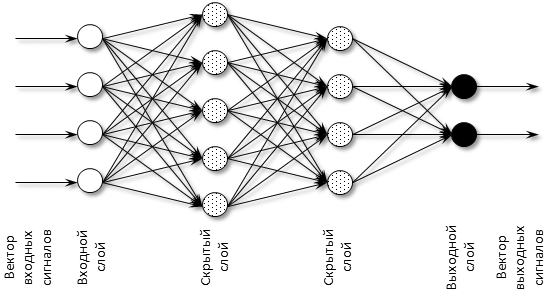
\includegraphics[width=0.7\textwidth]{nn_vizualisation.png}
  \caption{Нейронная сеть.}
  \label{fig:neuron}
\end{figure}
\end{frame}




\begin{frame}{Нейронные сети}
\begin{figure}[h]
    \centering
  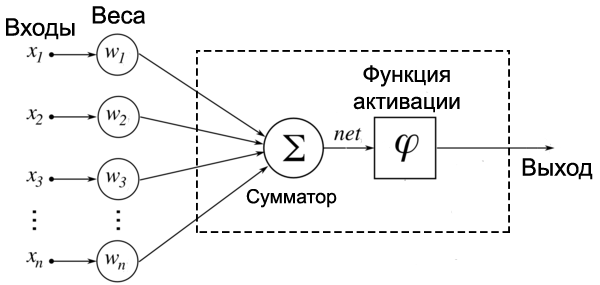
\includegraphics[width=0.7\textwidth]{nuron_model.png}
  \caption{Структура искусственного нейрона.}
  \label{fig:neuron}
\end{figure}
\end{frame}








\begin{frame}{Настройка Google Colaboratory}
\begin{figure}[h]
  \centering
  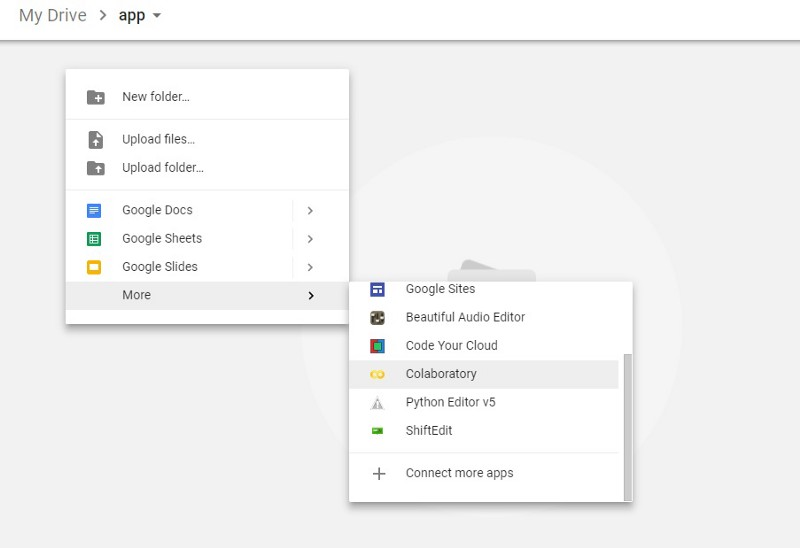
\includegraphics[width=0.7\textwidth]{colab_settings_1.jpeg} \\
  \caption{Создание файла.}
\end{figure}
\end{frame}





\begin{frame}{Настройка Google Colaboratory}
\begin{figure}[h]
  \centering
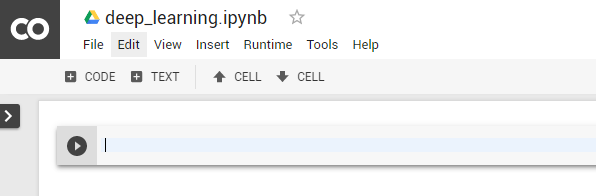
\includegraphics[width=0.7\textwidth]{colab_settings_3.png}    %лн
\end{figure}

\begin{figure}[h]
  \centering
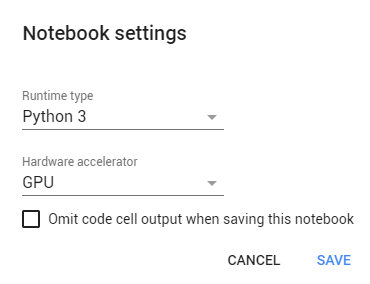
\includegraphics[width=0.5\textwidth]{colab_settings_2.png}\\    %пв
  \caption{Настройка GPU.}
\end{figure}
\end{frame}





\begin{frame}{Настройка Google Colaboratory}
\begin{figure}[h]
  \centering
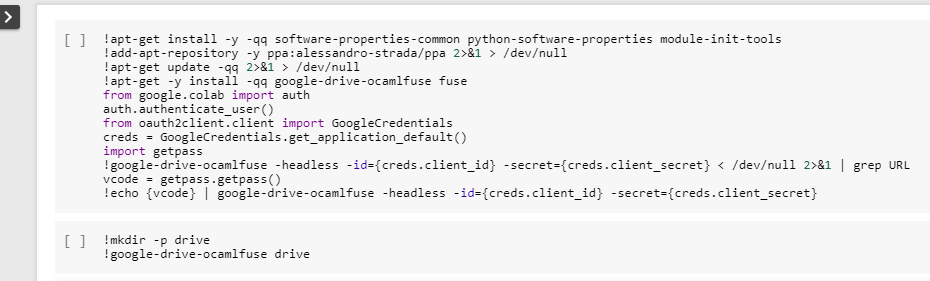
\includegraphics[width=0.8\textwidth]{colab_settings_4.png}    %пн
  \caption{Авторизация и подключение Google Drive.}
\end{figure}
\end{frame}





\begin{frame}{Построение набора данных}
\begin{block}{Информационные слова}
Сгенерируем все информационные слова из $\mathbb{F}_2^M$. Получим множество информационных слов $A = \{a_0; a_1; \dots; a_{M-1}\}$, где $a_i$ является двоичным представлением числа $i$ длины $n$.
\end{block}

\pause
\begin{block}{Кодовые слова}
Получим множество всех кодовых слов $\mathbb{C} = \{a\cdot G~|~\forall a \in A \}$. \\
Ясно, что~$|\mathbb{C}| = |A| = M$.
\end{block}
\pause
\begin{block}{Маски ошибок}
Создадим множество масок ошибок $E = \{e_0; \dots; e_n\}$.
\vspace*{-\baselineskip}
\begin{gather}
 % Remove numbering (before each equation)
    \nonumber e_0 = (0, 0, 0, 0, 0, 0, 0, 0, 0, 0, 0, 0, 0, 0, 0, 0), \\
    \nonumber e_1 = (1, 0, 0, 0, 0, 0, 0, 0, 0, 0, 0, 0, 0, 0, 0, 0), \\
    \nonumber \cdots \\
    \nonumber e_n = (0, 0, 0, 0, 0, 0, 0, 0, 0, 0, 0, 0, 0, 0, 0, 1).
\end{gather}
\end{block}

\end{frame}







\begin{frame}{Построение набора данных}
\begin{block}{Кодовые слова с ошибками}
Определим множество кодовых слов с ошибками $\widetilde{\mathbb{C}_i}$.
\begin{equation}
  \widetilde{\mathbb{C}_i} = \{c_i \oplus e ~|~  c_i \in \mathbb{C}~\space~\forall e \in E \}, где i \in \{0; \dots; M-1\}
\end{equation}
где $\oplus$ - операция сложения векторов по модулю $2$. Обозначим его элементы $\widetilde{c_i}$, где $i \in \{0; \dots; n\}$ - позиция единицы в образующей маске ошибки. Тогда $\widetilde{\mathbb{C}} = \bigcup\limits_{i=0}^{M-1} \widetilde{\mathbb{C}_i}$~-- множество всех кодовых слов с ошибками.
\end{block}
\pause

\begin{block}{Набор данных}
Определим блок $B_i = \{ (c_i, \widetilde{c}) ~|~ \forall~\widetilde{c} \in \widetilde{\mathbb{C}_i} \}, i \in \{0; \dots; M-1\}$. \\
Набор данных $D = \begin{pmatrix} B_0 \\ B_1 \\ \dots \\ B_{M-1} \end{pmatrix}$. Разобьем $D$ на $D_T$ и $D_V$ так: $\frac{D_V}{D_T}= \frac{30}{70}$.
\end{block}
\end{frame}









\begin{frame}{Параметры нейронной сети}
\begin{block}{Входные параметры}
Нейронная сеть получает на~вход ошибочное кодовое слово $\widetilde{c} \in \widetilde{\mathbb{C}}$,
где $\widetilde{c} = c \oplus e_j, c \in \mathbb{C}, j \in \{0;\dots; n\}$,
представленное в~виде набора признаков $f = (f_1, \dots, f_n)$, где~$f_i$ равен значению $i$-го бита~$\widetilde{c}$
\end{block}

\begin{block}{Выходные параметры}
Предполагается, что на выходе будет получено слово $\hat{c}$, с некоторой вероятностью равное слову $c$.
Слово $\hat{c}$ представляется вектором вероятностей~$p$. Каждый элемент $p_i~(\in [0, 1], i \in \{1;\dots; n\})$ вектора $p$, определяет вероятность того, что на~$i$-ой позиции слова $\hat{c}$ находится бит, равный единице.
\end{block}
\end{frame}







\begin{frame}{Параметры нейронной сети[2]}
\begin{block}{Гиперпараметры}
это такие параметры нейронной сети, которые не изменяются в процессе обучения нейронной сети, но от выбора которых зависит последующее качество работы сети.
\end{block}

\pause
\begin{block}{}
 \begin{itemize}
  \item Количество эпох обучения
  \item Количество слоев нейронной сети
  \item Количество нейронов в каждом слое
  \end{itemize}
\end{block}


\end{frame}




\begin{frame}{Параметры нейронной сети[3]}
\begin{block}{Функция потерь}
Функция потерь $f_{loss}(y, \hat{y})$ --- функция, характеризующая величину отклонения ответа $y$ нейронной сети от правильного ответа~$\hat{y}$.
\end{block}
\pause

 \begin{center}
Примеры: \quad $f_{log}(y, \hat{y}) = -\log(1 - |y-\hat{y}|)$,\qquad $f_{exp}(y, \hat{y}) = e^{|y-\hat{y}|} - 1$.
  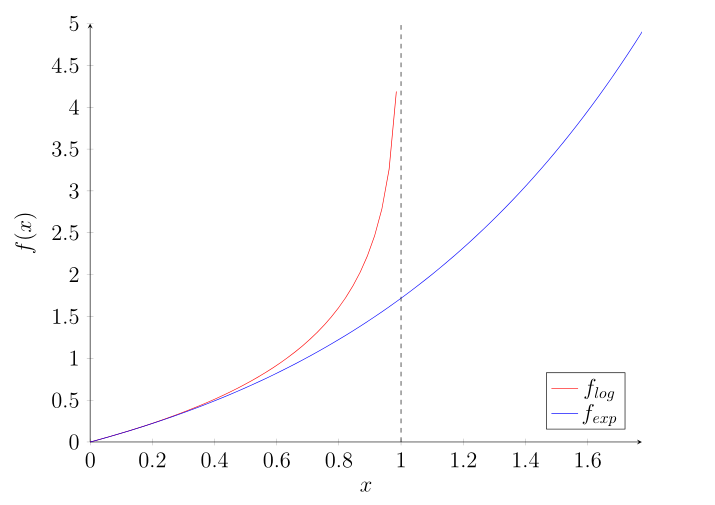
\includegraphics[width=0.5\textwidth]{losses_graphics.png}
 \end{center}

\end{frame}






\begin{frame}{Параметры нейронной сети[4]}
\begin{block}{Функция активации}
Функция активации $f_a(x)$ --- функция, вычисляющая выходной сигнал искусственного нейрона, где $x~=~\langle~W_i, x_{i-1}~\rangle$.
\end{block}

\begin{figure}[h]
    \centering
  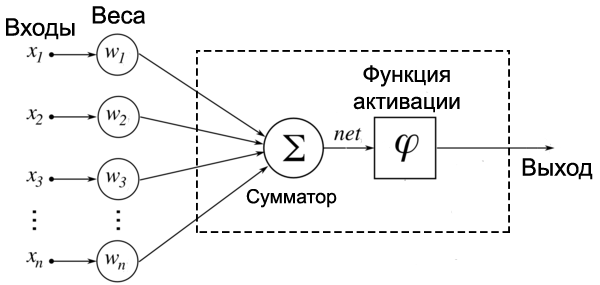
\includegraphics[width=0.5\textwidth]{nuron_model.png}
  \caption{Структура искусственного нейрона.}
  \label{fig:neuron}
\end{figure}

\end{frame}






\begin{frame}{Параметры нейронной сети[5]}
Примеры функций активации:
\begin{enumerate}
\item Функция единичного скачка
\item Линейный порог
\item Логистическая функция (сигмоид)
\item Гиперболический тангентс
\end{enumerate}

\begin{figure}[h]
    \centering
  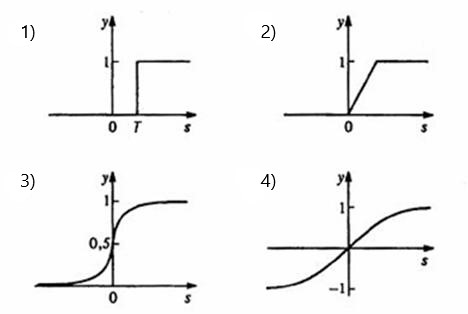
\includegraphics[width=0.5\textwidth]{activation_functions.jpg}
  \caption{Функции активации.}
  \label{fig:activations}
\end{figure}

\end{frame}









\begin{frame}{Выбор оптимальных гиперпараметров}
\begin{block}{}
\begin{itemize}
  \item hyperopt.fmin()
  \item keras.callbacks.History()
  \item keras.callbacks.ModelCheckpoint()
\end{itemize}
\end{block}

\pause
\begin{block}{Анализ результатов}
Наилучшее качество достигается при наборе гиперпараметров $s^*$, равном:
$$ s^* = \begin{cases} \mbox{Количество слоев} = 5, \\ \mbox{Количества нейронов} = 208, \\ \mbox{Размер батча} = 256, \\ f_{loss} = f_{exp}, \\ f_{a,i} = f_{sigmoid}. \end{cases}$$
\end{block}
\end{frame}






\begin{frame}{Построение нейронной сети}
\begin{figure}[h]
    \centering
    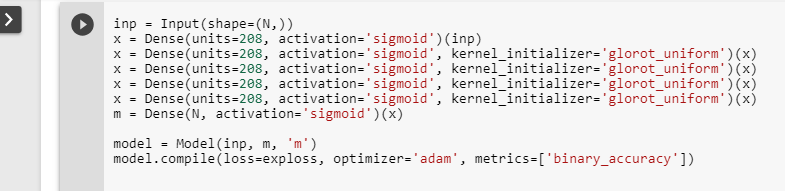
\includegraphics[width=0.8\textwidth]{neural_network_create.png}
    \caption{Создание модели нейронной сети.}
    \label{fig:neural_network_create}
\end{figure}


\begin{figure}[h]
    \centering
    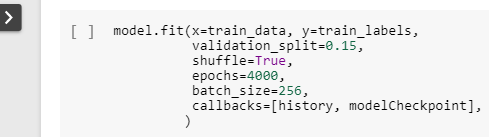
\includegraphics[width=0.7\textwidth]{neural_network_fit.png}
    \caption{Обучение модели.}
    \label{fig:neural_network_fir}
\end{figure}
\end{frame}








\begin{frame}{Графики обучения}

\begin{figure}[h]
    \centering
    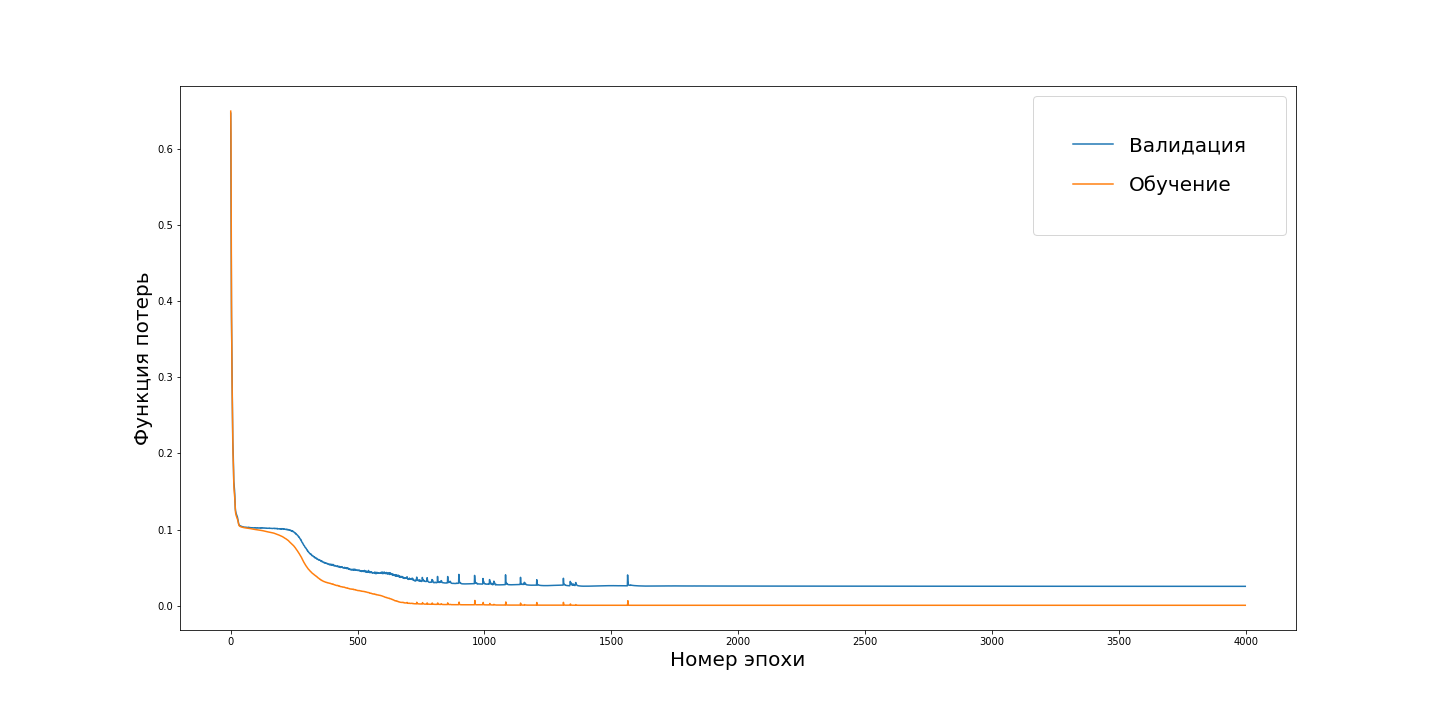
\includegraphics[scale=0.3]{model_loss}
    \caption{Функция потерь модели}
    \label{fig:loss}
\end{figure}

\end{frame}

\begin{frame}{Графики обучения}
\begin{figure}[h]
    \centering
    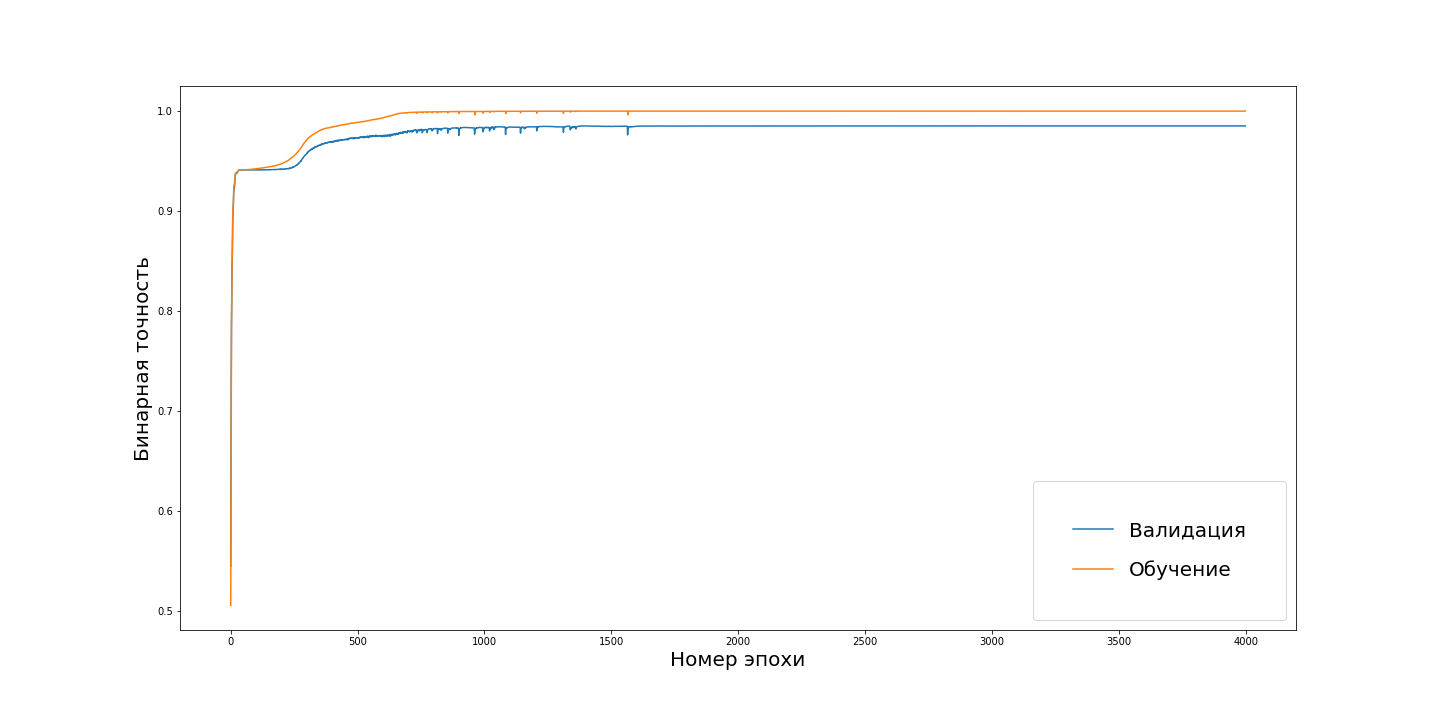
\includegraphics[scale=0.3]{model_binary_accuracy}
    \caption{Точность модели}
    \label{fig:accuracy}
\end{figure}

\end{frame}





\begin{frame}{Оценка качества}

\begin{block}{}
Определим функцию $eq(x, y) =
    \begin{cases}
            1, & \mbox{если } x~=~y, \\
        0, & \mbox{иначе}.
    \end{cases} $
\end{block}    

\begin{block}{}
Определим функцию $A(\mathcal{N}, D) = \frac{\sum\limits_{(c, \widetilde{c})\in D}eq(c, \mathcal{N}(\widetilde{c}))}{|D|}$.
\end{block}

\begin{block}{}
Проверка качества работы нейронной сети $\mathcal{N}$ с параметрами $s^*$ на валидационной выборке $D_V$ :
$$ A(\mathcal{N}_{s^*}, D_V)~\approx~0.92. $$

\end{block}
\end{frame}








\begin{frame}{Полученные результаты}

 \begin{itemize}
  \item {
    Построена реализация нейронной сети~$\mathcal{N}$, выполняющей декодирование кода~Хэмминга~$\mathcal{C}$ с~использованием технологии Google Colaboratory.
  }
  \item {
    Вероятность выдачи корректного результата работы нейронной сети~$\mathcal{N}$ равна~0.92.
  }
  \end{itemize}

\end{frame}





\end{document} 